% Options for packages loaded elsewhere
% Options for packages loaded elsewhere
\PassOptionsToPackage{unicode}{hyperref}
\PassOptionsToPackage{hyphens}{url}
\PassOptionsToPackage{dvipsnames,svgnames,x11names}{xcolor}
%
\documentclass[
  letterpaper,
  DIV=11,
  numbers=noendperiod]{scrartcl}
\usepackage{xcolor}
\usepackage{amsmath,amssymb}
\setcounter{secnumdepth}{-\maxdimen} % remove section numbering
\usepackage{iftex}
\ifPDFTeX
  \usepackage[T1]{fontenc}
  \usepackage[utf8]{inputenc}
  \usepackage{textcomp} % provide euro and other symbols
\else % if luatex or xetex
  \usepackage{unicode-math} % this also loads fontspec
  \defaultfontfeatures{Scale=MatchLowercase}
  \defaultfontfeatures[\rmfamily]{Ligatures=TeX,Scale=1}
\fi
\usepackage{lmodern}
\ifPDFTeX\else
  % xetex/luatex font selection
\fi
% Use upquote if available, for straight quotes in verbatim environments
\IfFileExists{upquote.sty}{\usepackage{upquote}}{}
\IfFileExists{microtype.sty}{% use microtype if available
  \usepackage[]{microtype}
  \UseMicrotypeSet[protrusion]{basicmath} % disable protrusion for tt fonts
}{}
\makeatletter
\@ifundefined{KOMAClassName}{% if non-KOMA class
  \IfFileExists{parskip.sty}{%
    \usepackage{parskip}
  }{% else
    \setlength{\parindent}{0pt}
    \setlength{\parskip}{6pt plus 2pt minus 1pt}}
}{% if KOMA class
  \KOMAoptions{parskip=half}}
\makeatother
% Make \paragraph and \subparagraph free-standing
\makeatletter
\ifx\paragraph\undefined\else
  \let\oldparagraph\paragraph
  \renewcommand{\paragraph}{
    \@ifstar
      \xxxParagraphStar
      \xxxParagraphNoStar
  }
  \newcommand{\xxxParagraphStar}[1]{\oldparagraph*{#1}\mbox{}}
  \newcommand{\xxxParagraphNoStar}[1]{\oldparagraph{#1}\mbox{}}
\fi
\ifx\subparagraph\undefined\else
  \let\oldsubparagraph\subparagraph
  \renewcommand{\subparagraph}{
    \@ifstar
      \xxxSubParagraphStar
      \xxxSubParagraphNoStar
  }
  \newcommand{\xxxSubParagraphStar}[1]{\oldsubparagraph*{#1}\mbox{}}
  \newcommand{\xxxSubParagraphNoStar}[1]{\oldsubparagraph{#1}\mbox{}}
\fi
\makeatother

\usepackage{color}
\usepackage{fancyvrb}
\newcommand{\VerbBar}{|}
\newcommand{\VERB}{\Verb[commandchars=\\\{\}]}
\DefineVerbatimEnvironment{Highlighting}{Verbatim}{commandchars=\\\{\}}
% Add ',fontsize=\small' for more characters per line
\usepackage{framed}
\definecolor{shadecolor}{RGB}{241,243,245}
\newenvironment{Shaded}{\begin{snugshade}}{\end{snugshade}}
\newcommand{\AlertTok}[1]{\textcolor[rgb]{0.68,0.00,0.00}{#1}}
\newcommand{\AnnotationTok}[1]{\textcolor[rgb]{0.37,0.37,0.37}{#1}}
\newcommand{\AttributeTok}[1]{\textcolor[rgb]{0.40,0.45,0.13}{#1}}
\newcommand{\BaseNTok}[1]{\textcolor[rgb]{0.68,0.00,0.00}{#1}}
\newcommand{\BuiltInTok}[1]{\textcolor[rgb]{0.00,0.23,0.31}{#1}}
\newcommand{\CharTok}[1]{\textcolor[rgb]{0.13,0.47,0.30}{#1}}
\newcommand{\CommentTok}[1]{\textcolor[rgb]{0.37,0.37,0.37}{#1}}
\newcommand{\CommentVarTok}[1]{\textcolor[rgb]{0.37,0.37,0.37}{\textit{#1}}}
\newcommand{\ConstantTok}[1]{\textcolor[rgb]{0.56,0.35,0.01}{#1}}
\newcommand{\ControlFlowTok}[1]{\textcolor[rgb]{0.00,0.23,0.31}{\textbf{#1}}}
\newcommand{\DataTypeTok}[1]{\textcolor[rgb]{0.68,0.00,0.00}{#1}}
\newcommand{\DecValTok}[1]{\textcolor[rgb]{0.68,0.00,0.00}{#1}}
\newcommand{\DocumentationTok}[1]{\textcolor[rgb]{0.37,0.37,0.37}{\textit{#1}}}
\newcommand{\ErrorTok}[1]{\textcolor[rgb]{0.68,0.00,0.00}{#1}}
\newcommand{\ExtensionTok}[1]{\textcolor[rgb]{0.00,0.23,0.31}{#1}}
\newcommand{\FloatTok}[1]{\textcolor[rgb]{0.68,0.00,0.00}{#1}}
\newcommand{\FunctionTok}[1]{\textcolor[rgb]{0.28,0.35,0.67}{#1}}
\newcommand{\ImportTok}[1]{\textcolor[rgb]{0.00,0.46,0.62}{#1}}
\newcommand{\InformationTok}[1]{\textcolor[rgb]{0.37,0.37,0.37}{#1}}
\newcommand{\KeywordTok}[1]{\textcolor[rgb]{0.00,0.23,0.31}{\textbf{#1}}}
\newcommand{\NormalTok}[1]{\textcolor[rgb]{0.00,0.23,0.31}{#1}}
\newcommand{\OperatorTok}[1]{\textcolor[rgb]{0.37,0.37,0.37}{#1}}
\newcommand{\OtherTok}[1]{\textcolor[rgb]{0.00,0.23,0.31}{#1}}
\newcommand{\PreprocessorTok}[1]{\textcolor[rgb]{0.68,0.00,0.00}{#1}}
\newcommand{\RegionMarkerTok}[1]{\textcolor[rgb]{0.00,0.23,0.31}{#1}}
\newcommand{\SpecialCharTok}[1]{\textcolor[rgb]{0.37,0.37,0.37}{#1}}
\newcommand{\SpecialStringTok}[1]{\textcolor[rgb]{0.13,0.47,0.30}{#1}}
\newcommand{\StringTok}[1]{\textcolor[rgb]{0.13,0.47,0.30}{#1}}
\newcommand{\VariableTok}[1]{\textcolor[rgb]{0.07,0.07,0.07}{#1}}
\newcommand{\VerbatimStringTok}[1]{\textcolor[rgb]{0.13,0.47,0.30}{#1}}
\newcommand{\WarningTok}[1]{\textcolor[rgb]{0.37,0.37,0.37}{\textit{#1}}}

\usepackage{longtable,booktabs,array}
\usepackage{calc} % for calculating minipage widths
% Correct order of tables after \paragraph or \subparagraph
\usepackage{etoolbox}
\makeatletter
\patchcmd\longtable{\par}{\if@noskipsec\mbox{}\fi\par}{}{}
\makeatother
% Allow footnotes in longtable head/foot
\IfFileExists{footnotehyper.sty}{\usepackage{footnotehyper}}{\usepackage{footnote}}
\makesavenoteenv{longtable}
\usepackage{graphicx}
\makeatletter
\newsavebox\pandoc@box
\newcommand*\pandocbounded[1]{% scales image to fit in text height/width
  \sbox\pandoc@box{#1}%
  \Gscale@div\@tempa{\textheight}{\dimexpr\ht\pandoc@box+\dp\pandoc@box\relax}%
  \Gscale@div\@tempb{\linewidth}{\wd\pandoc@box}%
  \ifdim\@tempb\p@<\@tempa\p@\let\@tempa\@tempb\fi% select the smaller of both
  \ifdim\@tempa\p@<\p@\scalebox{\@tempa}{\usebox\pandoc@box}%
  \else\usebox{\pandoc@box}%
  \fi%
}
% Set default figure placement to htbp
\def\fps@figure{htbp}
\makeatother


% definitions for citeproc citations
\NewDocumentCommand\citeproctext{}{}
\NewDocumentCommand\citeproc{mm}{%
  \begingroup\def\citeproctext{#2}\cite{#1}\endgroup}
\makeatletter
 % allow citations to break across lines
 \let\@cite@ofmt\@firstofone
 % avoid brackets around text for \cite:
 \def\@biblabel#1{}
 \def\@cite#1#2{{#1\if@tempswa , #2\fi}}
\makeatother
\newlength{\cslhangindent}
\setlength{\cslhangindent}{1.5em}
\newlength{\csllabelwidth}
\setlength{\csllabelwidth}{3em}
\newenvironment{CSLReferences}[2] % #1 hanging-indent, #2 entry-spacing
 {\begin{list}{}{%
  \setlength{\itemindent}{0pt}
  \setlength{\leftmargin}{0pt}
  \setlength{\parsep}{0pt}
  % turn on hanging indent if param 1 is 1
  \ifodd #1
   \setlength{\leftmargin}{\cslhangindent}
   \setlength{\itemindent}{-1\cslhangindent}
  \fi
  % set entry spacing
  \setlength{\itemsep}{#2\baselineskip}}}
 {\end{list}}
\usepackage{calc}
\newcommand{\CSLBlock}[1]{\hfill\break\parbox[t]{\linewidth}{\strut\ignorespaces#1\strut}}
\newcommand{\CSLLeftMargin}[1]{\parbox[t]{\csllabelwidth}{\strut#1\strut}}
\newcommand{\CSLRightInline}[1]{\parbox[t]{\linewidth - \csllabelwidth}{\strut#1\strut}}
\newcommand{\CSLIndent}[1]{\hspace{\cslhangindent}#1}



\setlength{\emergencystretch}{3em} % prevent overfull lines

\providecommand{\tightlist}{%
  \setlength{\itemsep}{0pt}\setlength{\parskip}{0pt}}



 


\usepackage{booktabs}
\usepackage{longtable}
\usepackage{array}
\usepackage{multirow}
\usepackage{wrapfig}
\usepackage{float}
\usepackage{colortbl}
\usepackage{pdflscape}
\usepackage{tabu}
\usepackage{threeparttable}
\usepackage{threeparttablex}
\usepackage[normalem]{ulem}
\usepackage{makecell}
\usepackage{xcolor}
\KOMAoption{captions}{tableheading}
\makeatletter
\@ifpackageloaded{caption}{}{\usepackage{caption}}
\AtBeginDocument{%
\ifdefined\contentsname
  \renewcommand*\contentsname{Table of contents}
\else
  \newcommand\contentsname{Table of contents}
\fi
\ifdefined\listfigurename
  \renewcommand*\listfigurename{List of Figures}
\else
  \newcommand\listfigurename{List of Figures}
\fi
\ifdefined\listtablename
  \renewcommand*\listtablename{List of Tables}
\else
  \newcommand\listtablename{List of Tables}
\fi
\ifdefined\figurename
  \renewcommand*\figurename{Figure}
\else
  \newcommand\figurename{Figure}
\fi
\ifdefined\tablename
  \renewcommand*\tablename{Table}
\else
  \newcommand\tablename{Table}
\fi
}
\@ifpackageloaded{float}{}{\usepackage{float}}
\floatstyle{ruled}
\@ifundefined{c@chapter}{\newfloat{codelisting}{h}{lop}}{\newfloat{codelisting}{h}{lop}[chapter]}
\floatname{codelisting}{Listing}
\newcommand*\listoflistings{\listof{codelisting}{List of Listings}}
\makeatother
\makeatletter
\makeatother
\makeatletter
\@ifpackageloaded{caption}{}{\usepackage{caption}}
\@ifpackageloaded{subcaption}{}{\usepackage{subcaption}}
\makeatother
\usepackage{bookmark}
\IfFileExists{xurl.sty}{\usepackage{xurl}}{} % add URL line breaks if available
\urlstyle{same}
\hypersetup{
  pdftitle={Coursework Template},
  pdfauthor={Jai Robinson},
  colorlinks=true,
  linkcolor={blue},
  filecolor={Maroon},
  citecolor={Blue},
  urlcolor={Blue},
  pdfcreator={LaTeX via pandoc}}


\title{Coursework Template}
\usepackage{etoolbox}
\makeatletter
\providecommand{\subtitle}[1]{% add subtitle to \maketitle
  \apptocmd{\@title}{\par {\large #1 \par}}{}{}
}
\makeatother
\subtitle{MSc in Statistics 2025/26, Imperial College London}
\author{Jai Robinson}
\date{}
\begin{document}
\maketitle


This Rmarkdown document is intended to provide a basic template that you
may use throughout the course, and to introduce you to basic
functionality of the open-source bookdown R package for writing
Rmarkdown documents (Xie 2016).

Please note:

\begin{itemize}
\tightlist
\item
  Rmarkdown syntax for the title and document style;
\item
  bookdown syntax to label and reference equations;
\item
  bookdown syntax to referencing literate and provide a bib file;
\item
  kable syntax to build clean and clear tables that can be referenced;
\item
  Rmarkdown inline functions to collect and print all code used.
\end{itemize}

\section{Sampling from the Cauchy
distribution}\label{sampling-from-the-cauchy-distribution}

In this question we seek to generate samples from the standard Cauchy
distribution, with pdf given by \begin{equation}
  p(x) = \frac{1}{\pi (1 + x^2)}, \quad x \in \mathbb{R}.
  (\#eq:1)
\end{equation} The cdf associated with @ref(eq:1) is given by
\begin{equation}
  F(x) = \frac{1}{\pi}\arctan(x) + \frac{1}{2}.
  (\#eq:2)
\end{equation}

\textbf{Part a.} We apply the inversion method as described by Graham
and Talay (2013). We first compute the generalised inverse of the cdf
@ref(eq:2). To this end, let \(y\in [0,1]\), then

\begin{align}
    y &= F(x), \quad \iff (\#eq:3a) \\
    y &= \frac{1}{\pi}\arctan(x) + \frac{1}{2} \quad \iff \\
    y-\frac{1}{2}  &= \frac{1}{\pi}\arctan(x)  \quad \iff \\
    \pi\left(y-\frac{1}{2}\right)  &= \arctan(x)  \quad \iff \\
    x &= \tan\left(\pi\left(y-\frac{1}{2}\right)\right). 
\end{align}

By the inversion method (Graham and Talay 2013), if \(Y \sim U[0,1]\),
then

\begin{equation}
  X = \tan\left(\pi\left(Y-\frac{1}{2}\right)\right),
  (\#eq:4)
\end{equation}

\textbf{Part b.} The empirical cdf based on \(N\) samples
\(x_1, \ldots, x_N\) is defined to be \[
                \widehat{F}(t) = \frac{1}{N}\sum_{i = 1}^N \mathbf{1}[x_i \leq t], \quad x\in \mathbb{t}.
              \] To generate the empirical cdf in R, we perform the
following steps:

\begin{enumerate}
\def\labelenumi{\alph{enumi}.}
\tightlist
\item
  Generate \(N\) samples from the distribution using the inversion
  method, as detailed in the previous question.\\
\item
  Sort the samples in ascending order
  \(x_1 \leq x_2 \leq x_3 \leq \ldots \leq x_N\).
\item
  The empirical CDF at value \(x_i\) is given by \(i/N\).
\end{enumerate}

In the following figure we plot the empirical cdf based on 1000 samples
(black line), and compare against the analytical cdf (red line).

\pandocbounded{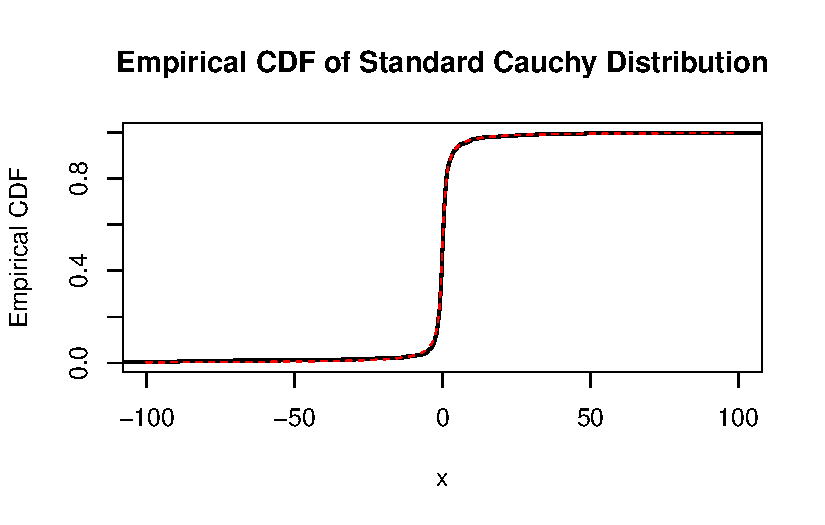
\includegraphics[keepaspectratio]{MSc_Statistics_coursework_quarto_files/figure-pdf/unnamed-chunk-2-1.pdf}}

\textbf{Part c.} We shall use the samples to compute the empirical cdf
for the values \(x = 0.5, 1, 10\).

\begin{table}
\centering
\caption{\label{tab:ecdf}Empirical CDF}
\centering
\fontsize{12}{14}\selectfont
\begin{tabular}[t]{r|r}
\hline
x & ecdf\\
\hline
0.5 & 0.64\\
\hline
1.0 & 0.75\\
\hline
10.0 & 0.97\\
\hline
\end{tabular}
\end{table}

\section{Code appendix}\label{code-appendix}

Rather than re-paste all the code to the appendix, here is a trick which
makes the markdown file output all the code (without) execution in the
appendix, without any duplication.

Please keep in mind to format the code so that the entire code is
clearly visible and does not run into the margins of the pdf version.

\begin{Shaded}
\begin{Highlighting}[]
\NormalTok{knitr}\SpecialCharTok{::}\NormalTok{opts\_chunk}\SpecialCharTok{$}\FunctionTok{set}\NormalTok{(}
  \AttributeTok{collapse =} \ConstantTok{TRUE}\NormalTok{,}
  \AttributeTok{comment =} \StringTok{"\#\textgreater{}"}
\NormalTok{)}
\NormalTok{include\_solutions }\OtherTok{\textless{}{-}} \ConstantTok{TRUE}
\FunctionTok{require}\NormalTok{(rmarkdown)}
\FunctionTok{require}\NormalTok{(knitr)}
\FunctionTok{require}\NormalTok{(kableExtra)}
\CommentTok{\# Put any library imports and other preamble here.}

\DocumentationTok{\#\#\# Question 1a}

\NormalTok{generate\_cauchy\_samples }\OtherTok{\textless{}{-}} \ControlFlowTok{function}\NormalTok{(n) \{}
  \CommentTok{\# Generate \textquotesingle{}n\textquotesingle{} uniform random numbers between 0 and 1}
\NormalTok{  u }\OtherTok{\textless{}{-}} \FunctionTok{runif}\NormalTok{(n)}
  
  \CommentTok{\# Apply the inverse CDF formula to get Cauchy samples}
\NormalTok{  samples }\OtherTok{\textless{}{-}} \FunctionTok{tan}\NormalTok{(pi }\SpecialCharTok{*}\NormalTok{ (u }\SpecialCharTok{{-}} \FloatTok{0.5}\NormalTok{))  }
  \FunctionTok{return}\NormalTok{(samples)}
\NormalTok{\}}

\NormalTok{num\_samples }\OtherTok{=} \DecValTok{1000}

\CommentTok{\# Generate samples from the standard Cauchy distribution}
\NormalTok{cauchy\_samples }\OtherTok{\textless{}{-}} \FunctionTok{generate\_cauchy\_samples}\NormalTok{(num\_samples)}


\DocumentationTok{\#\#\# Question 1b}

\CommentTok{\# Sort the samples in ascending order}
\NormalTok{sorted\_samples }\OtherTok{\textless{}{-}} \FunctionTok{sort}\NormalTok{(cauchy\_samples)}

\CommentTok{\# Calculate the cumulative probabilities for each sample}
\NormalTok{cumulative\_probs }\OtherTok{\textless{}{-}}\NormalTok{ (}\DecValTok{1}\SpecialCharTok{:}\NormalTok{num\_samples) }\SpecialCharTok{/}\NormalTok{ num\_samples}

\NormalTok{x\_values }\OtherTok{\textless{}{-}} \FunctionTok{seq}\NormalTok{(}\SpecialCharTok{{-}}\DecValTok{100}\NormalTok{, }\DecValTok{100}\NormalTok{,  }\AttributeTok{length.out =} \DecValTok{1000}\NormalTok{)}
\NormalTok{cdf\_values }\OtherTok{\textless{}{-}} \FunctionTok{pcauchy}\NormalTok{(x\_values)}

\CommentTok{\# Plot the empirical CDF}
\FunctionTok{plot}\NormalTok{(sorted\_samples, }
\NormalTok{     cumulative\_probs, }
     \AttributeTok{type =} \StringTok{"s"}\NormalTok{, }
     \AttributeTok{xlab =} \StringTok{"x"}\NormalTok{, }
     \AttributeTok{ylab =} \StringTok{"Empirical CDF"}\NormalTok{, }
     \AttributeTok{main =} \StringTok{"Empirical CDF of Standard Cauchy Distribution"}\NormalTok{, }
     \AttributeTok{lwd =} \DecValTok{2}\NormalTok{, }\AttributeTok{lty =} \DecValTok{1}\NormalTok{, }\AttributeTok{xlim =} \FunctionTok{c}\NormalTok{(}\SpecialCharTok{{-}}\DecValTok{100}\NormalTok{,}\DecValTok{100}\NormalTok{))}
\FunctionTok{lines}\NormalTok{(x\_values, cdf\_values, }\AttributeTok{type =} \StringTok{"l"}\NormalTok{, }
      \AttributeTok{xlab =} \StringTok{"x"}\NormalTok{, }\AttributeTok{ylab =} \StringTok{"CDF"}\NormalTok{, }\AttributeTok{main =} \StringTok{"CDF of Standard Cauchy Distribution"}\NormalTok{, }
      \AttributeTok{col =} \StringTok{\textquotesingle{}red\textquotesingle{}}\NormalTok{, }\AttributeTok{lty =} \DecValTok{2}\NormalTok{)}

\DocumentationTok{\#\#\# Question 1c}

\NormalTok{calculate\_ecdf }\OtherTok{\textless{}{-}} \ControlFlowTok{function}\NormalTok{(x) \{}
    \FunctionTok{return}\NormalTok{(}\FunctionTok{sum}\NormalTok{(sorted\_samples }\SpecialCharTok{\textless{}=}\NormalTok{ x)}\SpecialCharTok{/}\NormalTok{num\_samples)}
\NormalTok{\}}

\NormalTok{df }\OtherTok{\textless{}{-}} \FunctionTok{data.frame}\NormalTok{(}\AttributeTok{x =} \FunctionTok{c}\NormalTok{(}\FloatTok{0.5}\NormalTok{, }\FloatTok{1.0}\NormalTok{, }\FloatTok{10.0}\NormalTok{), }
                \AttributeTok{ecdf =} \FunctionTok{c}\NormalTok{(}\FunctionTok{calculate\_ecdf}\NormalTok{(}\FloatTok{0.5}\NormalTok{), }
                         \FunctionTok{calculate\_ecdf}\NormalTok{(}\FloatTok{1.0}\NormalTok{), }
                         \FunctionTok{calculate\_ecdf}\NormalTok{(}\FloatTok{10.0}\NormalTok{))}
\NormalTok{                )}
\FunctionTok{kbl}\NormalTok{(df,}
    \AttributeTok{caption =} \StringTok{\textquotesingle{}Empirical CDF\textquotesingle{}}\NormalTok{, }
    \AttributeTok{label =} \StringTok{\textquotesingle{}ecdf\textquotesingle{}}\NormalTok{,}
    \AttributeTok{digits =} \DecValTok{2}\NormalTok{) }\SpecialCharTok{\%\textgreater{}\%}
  \FunctionTok{kable\_styling}\NormalTok{(}
    \AttributeTok{bootstrap\_options =} \FunctionTok{c}\NormalTok{(}\StringTok{"striped"}\NormalTok{, }\StringTok{"hover"}\NormalTok{, }\StringTok{"condensed"}\NormalTok{),}
    \AttributeTok{font\_size =} \DecValTok{12}\NormalTok{)}
\end{Highlighting}
\end{Shaded}

\section*{References}\label{references}
\addcontentsline{toc}{section}{References}

\phantomsection\label{refs}
\begin{CSLReferences}{1}{0}
\bibitem[\citeproctext]{ref-graham2013stochastic}
Graham, Carl, and Denis Talay. 2013. \emph{Stochastic Simulation and
Monte Carlo Methods: Mathematical Foundations of Stochastic Simulation}.
Vol. 68. Springer Science \& Business Media.

\bibitem[\citeproctext]{ref-xie2016bookdown}
Xie, Yihui. 2016. \emph{Bookdown: Authoring Books and Technical
Documents with r Markdown}. CRC Press.

\end{CSLReferences}




\end{document}
